\documentclass[aspectratio=169]{beamer}

\usepackage{graphicx}
\usepackage{subcaption}
\usepackage{bm}

\title{TRC 2019 Project 2 WP 2 Meeting 5}
\author{Eve, Nidish, Paw}

\begin{document}
\maketitle{}

\begin{frame}
  \frametitle{Overview}
  \begin{itemize}
  \item Have been training PNLSS using Multisine data with frequencies
    around the 1st, 2nd, and 3rd modes separately as well as together
  \item Primary focus here is on benchmarks 2 \& 3
  \item The BLA is able to predict well that the number of states
    required is 6 for the simulations
  \item Have also tried to implement the shaker model along with the
    HB simulations, but here EPMC does not seem to get the correct
    results
  \item I'm implementing the phase-resonance condition as an extra
    equation for this currently
  \end{itemize}
\end{frame}

\begin{frame}[allowframebreaks]
  \frametitle{Benchmark 2}

  \begin{figure}
    \centering
    \begin{subfigure}{0.5\linewidth}
      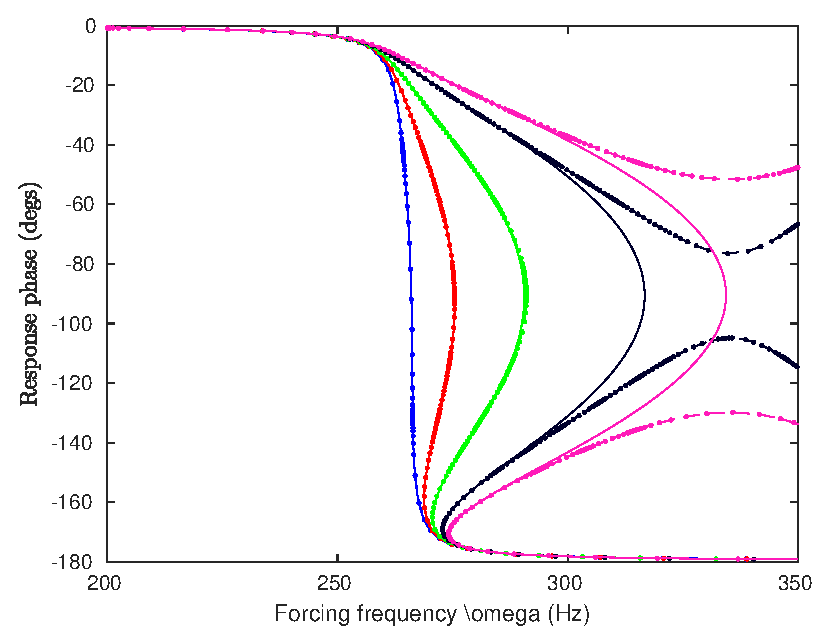
\includegraphics[width=\linewidth]{{../../../benchmark2/fig/pnlssfrf_A0.01_Phase_nx3_mds1}.eps}
      \caption{u=0.01}
    \end{subfigure}%
    \begin{subfigure}{0.5\linewidth}
      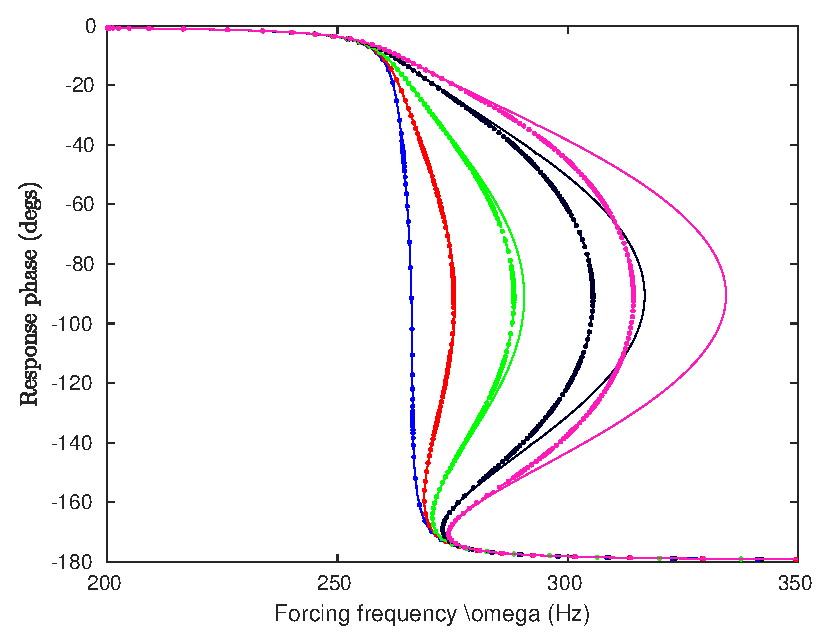
\includegraphics[width=\linewidth]{{../../../benchmark2/fig/pnlssfrf_A0.05_Phase_nx3_mds1}.eps}
      \caption{u=0.05}
    \end{subfigure}

    \begin{subfigure}{0.5\linewidth}
      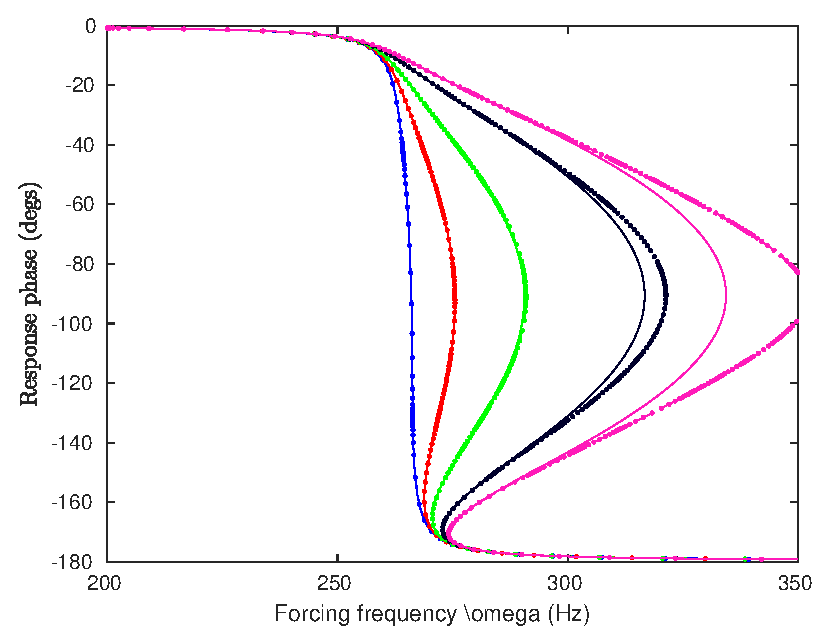
\includegraphics[width=\linewidth]{{../../../benchmark2/fig/pnlssfrf_A0.10_Phase_nx3_mds1}.eps}
      \caption{u=0.10}
    \end{subfigure}%
    \begin{subfigure}{0.5\linewidth}
      \includegraphics[width=\linewidth]{{../../../benchmark2/fig/pnlssfrf_A0.15_Phase_nx3_mds1}.eps}
      \caption{u=0.15}
    \end{subfigure}

    \begin{subfigure}{0.5\linewidth}
      \includegraphics[width=\linewidth]{{../../../benchmark2/fig/pnlssfrf_A0.20_Phase_nx3_mds1}.eps}
      \caption{u=0.20}
    \end{subfigure}%
    \begin{subfigure}{0.5\linewidth}
      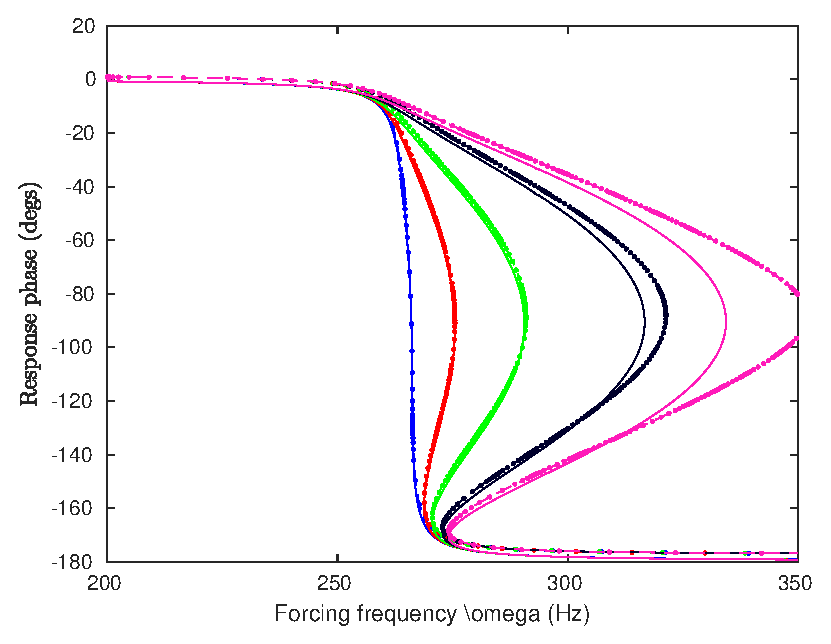
\includegraphics[width=\linewidth]{{../../../benchmark2/fig/pnlssfrf_A0.25_Phase_nx3_mds1}.eps}
      \caption{u=0.25}
    \end{subfigure}    
  \end{figure}
\end{frame}

% \begin{frame}[allowframebreaks]
%   \frametitle{Benchmark 2}
%   \framesubtitle{Single Mode Excitation}
%   \textbf{Mode 1}
%   \begin{figure}
%     \centering
%     \begin{subfigure}{0.5\linewidth}
%       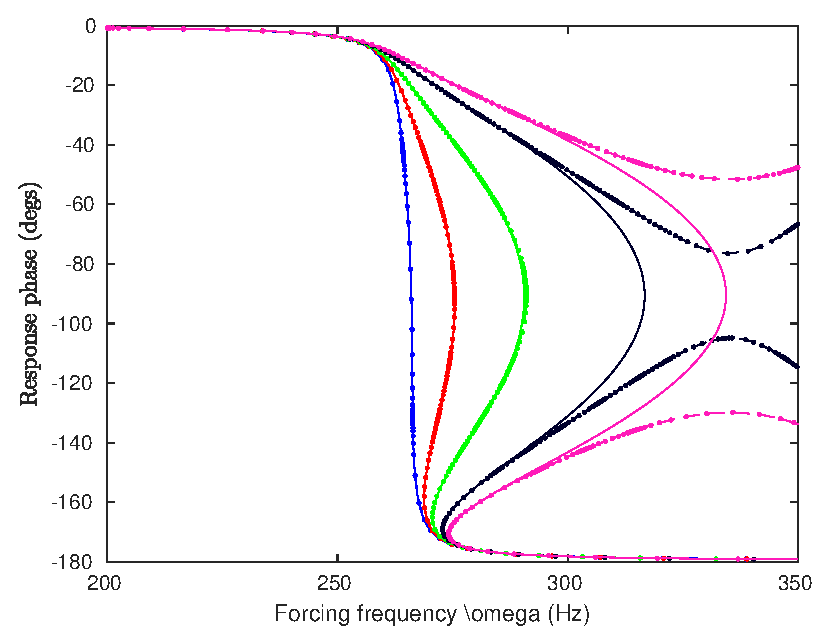
\includegraphics[width=\linewidth]{{../../../benchmark2/fig/pnlssfrf_A0.01_Phase_nx3_mds1}.eps}
%       \capttion{u=0.01}
%     \end{subfigure}%
%     \begin{subfigure}{0.5\linewidth}
%       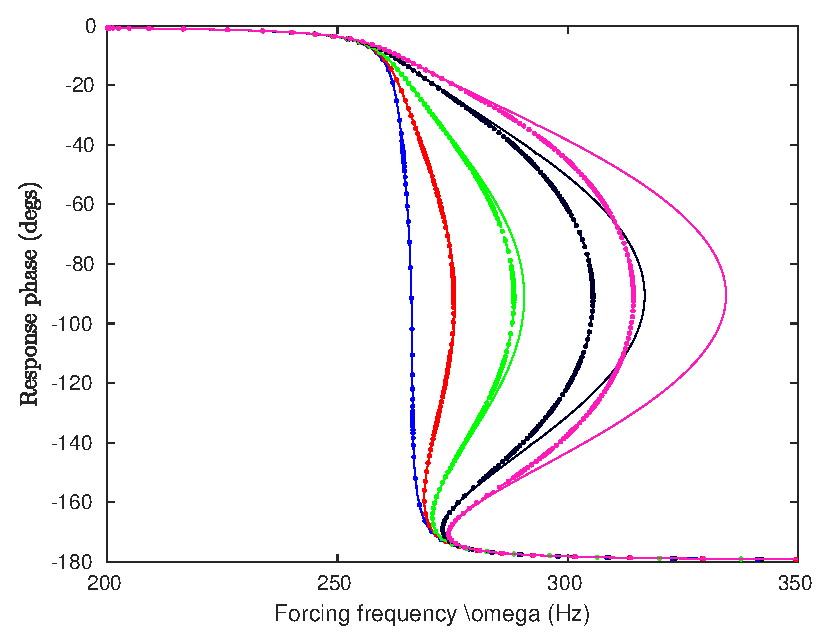
\includegraphics[width=\linewidth]{{../../../benchmark2/fig/pnlssfrf_A0.05_Phase_nx3_mds1}.eps}
%       \caption{u=0.05}
%     \end{subfigure}
%     \begin{subfigure}{0.5\linewidth}
%       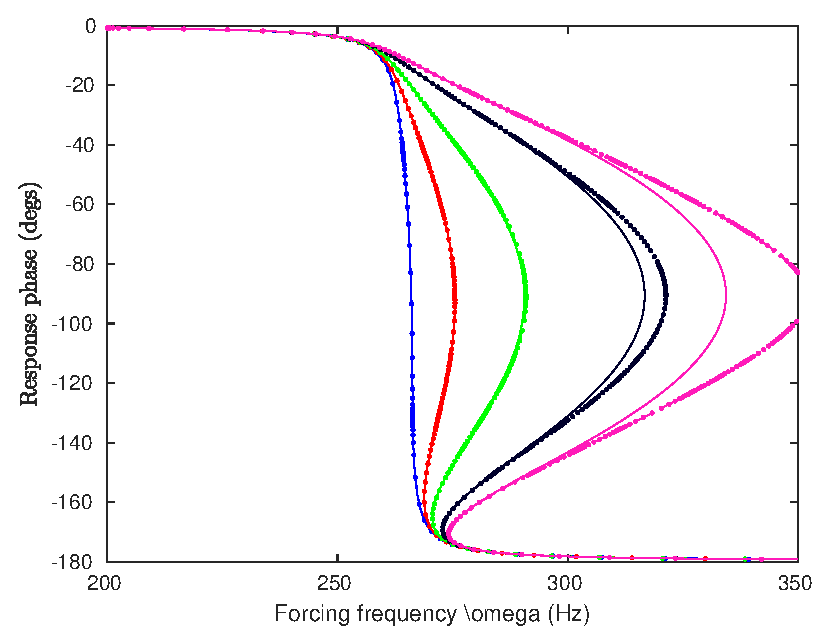
\includegraphics[width=\linewidth]{{../../../benchmark2/fig/pnlssfrf_A0.10_Phase_nx3_mds1}.eps}
%       \capttion{u=0.10}
%     \end{subfigure}%
%     \begin{subfigure}{0.5\linewidth}
%       \includegraphics[width=\linewidth]{{../../../benchmark2/fig/pnlssfrf_A0.15_Phase_nx3_mds1}.eps}
%       \caption{u=0.15}
%     \end{subfigure}

%     \begin{subfigure}{0.5\linewidth}
%       \includegraphics[width=\linewidth]{{../../../benchmark2/fig/pnlssfrf_A0.20_Phase_nx3_mds1}.eps}
%       \capttion{u=0.20}
%     \end{subfigure}%
%     \begin{subfigure}{0.5\linewidth}
%       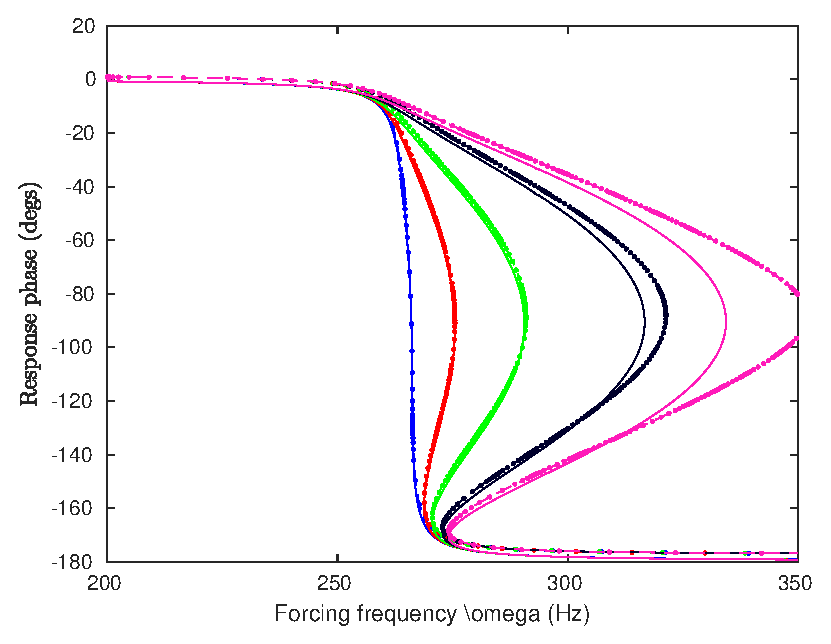
\includegraphics[width=\linewidth]{{../../../benchmark2/fig/pnlssfrf_A0.25_Phase_nx3_mds1}.eps}
%       \caption{u=0.25}
%     \end{subfigure}
%   \end{figure}

%   % \textbf{Mode 1, 2, 3 (Simultaneously)}
%   % \begin{figure}
%   %   \centering
%   %   \begin{subfigure}{0.5\linewidth}
%   %     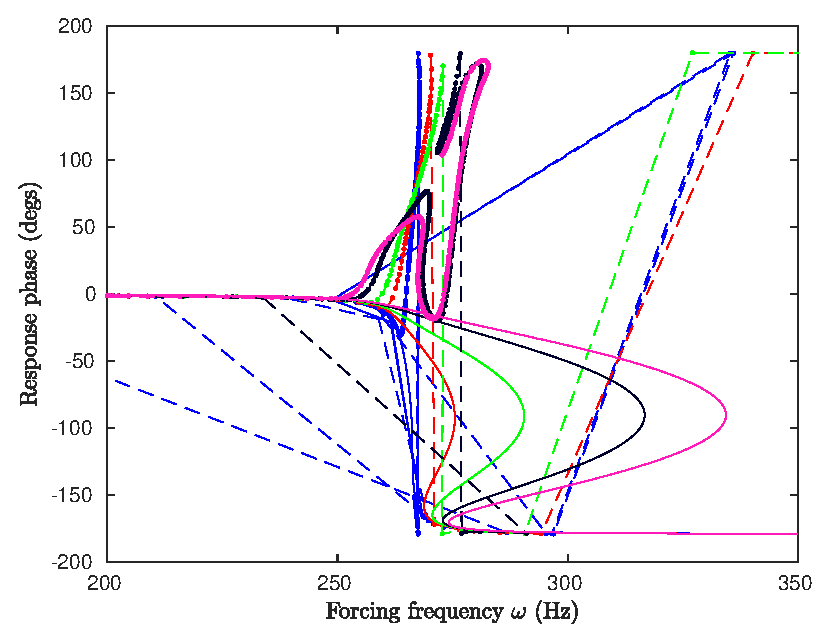
\includegraphics[width=\linewidth]{{../../../benchmark2/fig/pnlssfrf_A0.01_Phase_nx3_mds123}.eps}
%   %     \capttion{u=0.01}
%   %   \end{subfigure}%
%   %   \begin{subfigure}{0.5\linewidth}
%   %     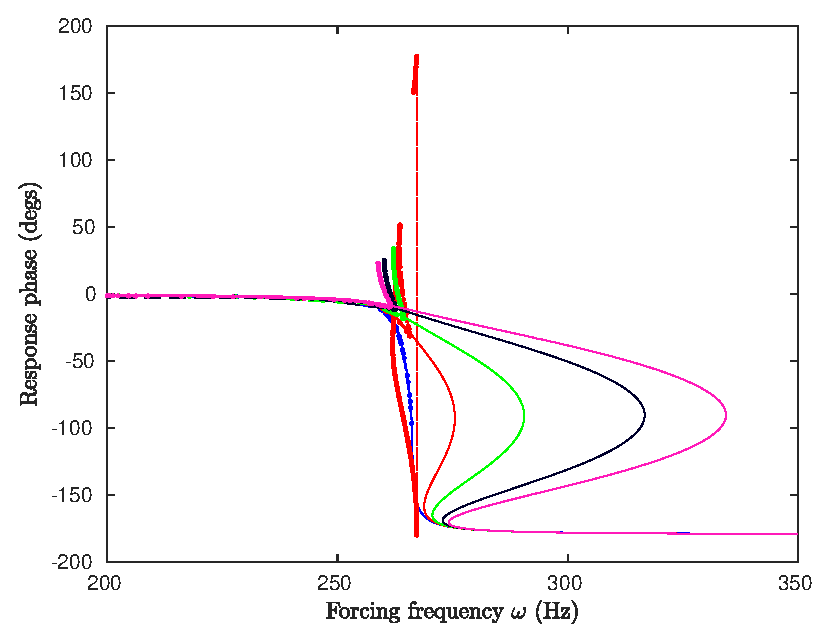
\includegraphics[width=\linewidth]{{../../../benchmark2/fig/pnlssfrf_A0.05_Phase_nx3_mds123}.eps}
%   %     \caption{u=0.05}
%   %   \end{subfigure}

%   %   \begin{subfigure}{0.5\linewidth}
%   %     \includegraphics[width=\linewidth]{{../../../benchmark2/fig/pnlssfrf_A0.10_Phase_nx3_mds123}.eps}
%   %     \capttion{u=0.10}
%   %   \end{subfigure}%
%   %   \begin{subfigure}{0.5\linewidth}
%   %     \includegraphics[width=\linewidth]{{../../../benchmark2/fig/pnlssfrf_A0.15_Phase_nx3_mds123}.eps}
%   %     \caption{u=0.15}
%   %   \end{subfigure}

%   %   \begin{subfigure}{0.5\linewidth}
%   %     \includegraphics[width=\linewidth]{{../../../benchmark2/fig/pnlssfrf_A0.20_Phase_nx3_mds123}.eps}
%   %     \capttion{u=0.20}
%   %   \end{subfigure}%
%   %   \begin{subfigure}{0.5\linewidth}
%   %     \includegraphics[width=\linewidth]{{../../../benchmark2/fig/pnlssfrf_A0.25_Phase_nx3_mds123}.eps}
%   %     \caption{u=0.25}
%   %   \end{subfigure}
% %   \end{figure}
% % \end{frame}
%   \end{figure}
% \end{frame}

\end{document}
%%% Local Variables:
%%% mode: latex
%%% TeX-master: t
%%% End:
